\documentclass{beamer}


% Beamer settings
\usecolortheme{rose}
\beamertemplatenavigationsymbolsempty
\setbeamertemplate{footline}[frame number]

\titlegraphic{%

\includegraphics[height=1cm]{logo-full-colour.png}}

\addtobeamertemplate{frametitle}{}{%
\begin{tikzpicture}[remember picture,overlay]
\node[anchor=north east,yshift=2pt] at (current page.north east) {
\includegraphics[height=1cm]{logo-full-colour.png}};
\end{tikzpicture}}

% Packages
\usepackage{amsmath}

\usepackage{tikz}
\usetikzlibrary{positioning}
\usetikzlibrary{fit}

\usepackage{pgfplots}
\usepgfplotslibrary{fillbetween}

\usepackage{minted}
\usepackage[T1]{fontenc} % Required by minted to ensure dollar signs are produced instead of pound (sterling) signs

\usepackage{multicol}

\usepackage{booktabs}

\usepackage{adjustbox}

% Author
\author{Simon McIntosh-Smith \& Tom Deakin\\University of Bristol}

\date{}



\title{OpenMP for Computational Scientists}
\subtitle{4: Combining MPI and OpenMP}

\begin{document}

\frame{\titlepage}

%-------------------------------------------------------------------------------
\begin{frame}
\frametitle{Outline}
\begin{itemize}
  \item Non-uniform Memory Access
  \item Thread affinity in OpenMP
  \item Combining MPI with OpenMP
\end{itemize}
\end{frame}

%-------------------------------------------------------------------------------
\begin{frame}
\frametitle{NUMA}
\end{frame}

%-------------------------------------------------------------------------------
\begin{frame}
\frametitle{OpenMP proc bind}
\end{frame}

%-------------------------------------------------------------------------------
\begin{frame}
\frametitle{Why combine MPI+OpenMP}
Include scaling results
\begin{itemize}
  \item Larger fewer messages
  \item Fewer MPI ranks
  \item Parallelise other dimension not decomposed with MPI
\end{itemize}
\end{frame}

%-------------------------------------------------------------------------------
\begin{frame}[fragile]
\frametitle{MPI programs}
What happens when you run an MPI program?
\begin{minted}{bash}
mpirun -np 16 ./a.out
\end{minted}

\begin{itemize}
  \item 16 processes are spawned on one (or more) nodes according to the hostname list file given by the queueing system.
    \begin{itemize}
      \item E.g. with PBS (\mintinline{bash}|qsub|, etc.) set by \mintinline{bash}|$PBS_NODEFILE|.
    \end{itemize}
  \item There is no reason why these processes have to be serial:
  \begin{itemize}
    \item Each MPI rank could spawn OpenMP threads and run in parallel.
    \item Each MPI rank could use a GPU.
  \end{itemize}
\end{itemize}

\end{frame}

%-------------------------------------------------------------------------------
\begin{frame}[fragile]
\frametitle{Compiling OpenMP and MPI code}
\begin{itemize}
  \item Remember building MPI code just uses a the wrapper commands.
  \item Just pass in the OpenMP flag as usual:
    \begin{itemize}
      \item GNU: \mintinline{bash}|mpif90| -fopenmp
      \item Intel: \mintinline{bash}|mpiifort| -qopenmp
      \item Cray: \mintinline{bash}|ftn|
    \end{itemize}
  \item Set the number of OpenMP threads \emph{per rank}.
  \item E.g 2 MPI ranks, 8 threads per rank:
  \begin{minted}{bash}
  OMP_NUM_THREADS=8 mpirun -np 2 ./a.out
  \end{minted}
\end{itemize}
\end{frame}

%-------------------------------------------------------------------------------
\begin{frame}[fragile]
\frametitle{Combining OpenMP and MPI}
\begin{itemize}
  \item MPI assumes that each MPI process does not spawn anything else.
  \item Must initilise MPI differently if using threads!
  \begin{minted}{fortran}
  call MPI_Init_thread(required, provided, ierr)
  \end{minted}

  \item You specify a required thread support level, and it returns the the level it could support.
  \item A good idea to check \mintinline{fortran}|provided .ge. required|.
\end{itemize}
\end{frame}

%-------------------------------------------------------------------------------
\begin{frame}
\frametitle{Thread support levels}
\begin{itemize}
  \item \mintinline{fortran}|MPI_THREAD_SINGLE| \\
  Only one thread will execute (no threads allowed).

  \item \mintinline{fortran}|MPI_THREAD_FUNNELED| \\
  May spawn threads, but only the original process may call MPI routines: the one that called \mintinline{fortran}|MPI_Init|.

  \item \mintinline{fortran}|MPI_THREAD_SERIALIZED| \\
  May spawn threads and any thread can make MPI calls, but only one at a time. \emph{Your} responsibility to synchronise.

  \item \mintinline{fortran}|MPI_THREAD_MULTIPLE| \\
  May spawn threads and any thread can make MPI calls. The MPI library has to deal with being called in parallel.
\end{itemize}

\end{frame}

%-------------------------------------------------------------------------------
\begin{frame}[fragile]
\frametitle{Example: MPI\_THREAD\_FUNNELED}
Only the original process is allowed to call MPI routines.
\begin{minted}[frame=single]{fortran}
!$omp parallel
... ! Parallel work
!$omp end parallel
call MPI_Sendrecv()
\end{minted}
\end{frame}

%-------------------------------------------------------------------------------
\begin{frame}[fragile]
\frametitle{MPI\_THREAD\_SERIALIZED}
The threads are allowed to call MPI, but you must program in synchronisation to ensure only one thread calls MPI at a time.
\begin{minted}[frame=single]{fortran}
!$omp parallel
  ... ! Parallel work
  !$omp critical
  call MPI_Sendrecv()
  !$omp end critical
!$omp end parallel
\end{minted}
\end{frame}

%-------------------------------------------------------------------------------
\begin{frame}[fragile]
\frametitle{MPI\_THREAD\_MULTIPLE}
Any thread can call MPI whenever it likes. The \mintinline{fortran}|MPI_THREAD_MULTIPLE| guarantees the MPI library will be OK with this.
\begin{minted}[frame=single]{fortran}
!$omp parallel
  ... ! Parallel work
  call MPI_Sendrecv()
!$omp end parallel
\end{minted}
\end{frame}

%-------------------------------------------------------------------------------
\begin{frame}
\frametitle{MPI library thread support}
\begin{itemize}
  \item Intel
  \item OpenMPI
  \item MPICH
  \item Cray
\end{itemize}
\end{frame}

%-------------------------------------------------------------------------------
\begin{frame}
\frametitle{Thread pinning}
\begin{itemize}
  \item Need to be very careful how MPI ranks and OpenMP threads are mapped to the physical hardware.
  \item Imagine 2 dual-socket nodes: 4 sockets with (say) 16 cores per socket.
  \item Launch 64 MPI ranks: 1 per core.
    \begin{itemize}
      \item This is flat MPI.
      \item Launching OpenMP threads will overallocate threads compared to hardware resource.
      \item Warning: things will slow down.
    \end{itemize}
  \item Launch 4 MPI ranks (one per socket).
    \begin{itemize}
      \item Leaves 16 cores per MPI rank for OpenMP threads to run on.
      \item But need to make sure threads go to the right places!
      \item Often close interaction with the queuing system --- system dependant behaviour.
    \end{itemize}
\end{itemize}
\end{frame}

%-------------------------------------------------------------------------------
\begin{frame}[fragile]
\frametitle{Example: default placement}
Example MPI rank placement with standard PBS setup.

\begin{minted}{bash}
mpirun -np 4 ./a.out
\end{minted}

\begin{center}
\begin{adjustbox}{max width={\textwidth}}

\begin{tikzpicture}

  \foreach \loc in {0, 3, 7, 10} {
  \foreach \i in {0,...,1} {
    \foreach \j in {0,...,1} {
      \draw (\loc+\i,\j) rectangle (\loc+\i+1,\j+1);
    }
  }
  }

  \draw[dashed] (-0.5,-0.5) rectangle (5.5,2.5);
  \draw[dashed] (6.5,-0.5) rectangle (12.5,2.5);

  \foreach \i in {0,...,1} {
    \foreach \j in {0,...,1} {
      \draw<2->[fill=red] (3+\i+.5,\j+.5) circle (0.4cm);
    }
  }
\end{tikzpicture}
\end{adjustbox}
\end{center}
\onslide<2->{
 All ranks placed on the second socket of the first node.
}
\end{frame}

%-------------------------------------------------------------------------------

\begin{frame}[fragile]
\frametitle{Example: pin MPI to one core per socket}
\begin{itemize}
  \item Tell the OS and MPI runtime to pin each MPI to the first core in each socket.
  \item For OpenMPI:
  \begin{minted}{bash}
  export OMP_NUM_THREADS=4
  mpirun -np 4 --npersocket 1 ./a.out
  \end{minted}
  \item Where do the threads go?
\end{itemize}


\begin{center}
\begin{adjustbox}{max width={\textwidth}}
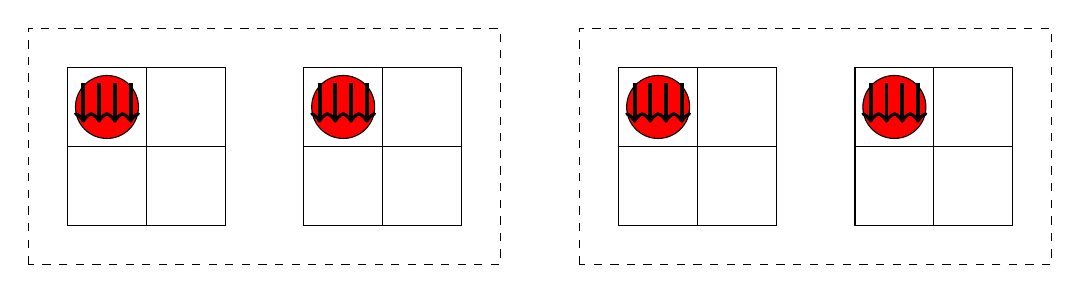
\begin{tikzpicture}

  \foreach \loc in {0, 3, 7, 10} {
  \foreach \i in {0,...,1} {
    \foreach \j in {0,...,1} {
      \draw (\loc+\i,\j) rectangle (\loc+\i+1,\j+1);
    }
  }
  }

  \draw[dashed] (-0.5,-0.5) rectangle (5.5,2.5);
  \draw[dashed] (6.5,-0.5) rectangle (12.5,2.5);

  \foreach \i in {0, 3, 7, 10} {
    \draw[fill=red] (\i+0.5,1.5) circle (0.4cm);
    \foreach \j in {0.2, 0.4, 0.6, 0.8} {
      \draw<2->[->,line width=.5mm] (\i+\j,1.8) -- (\i+\j, 1.3);
    }
  }
\end{tikzpicture}
\end{adjustbox}
\end{center}

\onslide<2->{
Threads spawned inherit their parent's binding, which was one core.

Use \mintinline{bash}|--report-bindings| flag to see what's being pinned where.

}

\end{frame}

%-------------------------------------------------------------------------------
\begin{frame}
\frametitle{Example: pin MPI to socket}
\begin{itemize}
  \item Pin each MPI to cores on a socket, then OpenMP threads can spawn across the socket.
  \item OpenMPI gives three ways to do this:
  \begin{itemize}
    \item \mintinline{bash}|--bind-to-socket|
    \item \mintinline{bash}|--bind-to-core --cpus-per-proc 8|
    \item \mintinline{bash}|--map-by socket:PE=8| (v1.10 and up)
  \end{itemize}
\end{itemize}
\end{frame}

%-------------------------------------------------------------------------------
\begin{frame}
\frametitle{Pinning with Intel and Cray}
\begin{itemize}
  \item Intel MPI will need different flags and environment variables, but tends to do the right thing by default.
  \item Cray MPI (MVAPICH) can be controlled using \mintinline{bash}|aprun|.
  \item Cray MPI with the Intel compiler needs a different set of \mintinline{bash}|aprun| flags.
\end{itemize}
\end{frame}

%-------------------------------------------------------------------------------

\end{document}

